%
% Copyright (c) 2016 Intel Corporation
%
% Permission is hereby granted, free of charge, to any person obtaining a copy
% of this software and associated documentation files (the "Software"), to
% deal in the Software without restriction, including without limitation the
% rights to use, copy, modify, merge, publish, distribute, sublicense, and/or
% sell copies of the Software, and to permit persons to whom the Software is
% furnished to do so, subject to the following conditions:
%
% The above copyright notice and this permission notice shall be included in
% all copies or substantial portions of the Software.
%
% THE SOFTWARE IS PROVIDED "AS IS", WITHOUT WARRANTY OF ANY KIND, EXPRESS OR
% IMPLIED, INCLUDING BUT NOT LIMITED TO THE WARRANTIES OF MERCHANTABILITY,
% FITNESS FOR A PARTICULAR PURPOSE AND NONINFRINGEMENT. IN NO EVENT SHALL THE
% AUTHORS OR COPYRIGHT HOLDERS BE LIABLE FOR ANY CLAIM, DAMAGES OR OTHER
% LIABILITY, WHETHER IN AN ACTION OF CONTRACT, TORT OR OTHERWISE, ARISING
% FROM, OUT OF OR IN CONNECTION WITH THE SOFTWARE OR THE USE OR OTHER DEALINGS
% IN THE SOFTWARE.
%
\documentclass{article}

% so we can insert images into the document
\usepackage{graphicx}
% this is where our image sources reside
\graphicspath{ {images/} }

% so we can the \subfigure environment
\usepackage{subcaption}

% so we can easily change the page margins
\usepackage{geometry}
\geometry{
	letterpaper,
	portrait,
	left=0.75in,
	right=0.75in,
	top=0.75in,
	bottom=0.75in,
}

% so we can use 'H' to strictly position figures
\usepackage{float}

% so we can use inline \textquote
\usepackage{csquotes}

% so we can import code listings from source files
\usepackage{listings}

% so we can get automatic cross referencing for most objects
\usepackage{hyperref}
\hypersetup{
    colorlinks=true,
    linkcolor=blue,
    filecolor=magenta,      
    urlcolor=cyan,
    %bookmarks=true, %--this is already invoked by default
}

% declare the attributes for our title
\title{HOWTO Supplemental Reset Components for Qsys}
\author{}
\date{
Document Revision 1.0
\newline
\newline
Built on \today
\newline
}

\begin{document}

% insert the default title format using our attributes
\maketitle

% make an entry in the PDF bookmarks for the TOC
\pdfbookmark[0]{Contents}{sumario_label}
% insert the default TOC format
\tableofcontents

%-------------------------------------------------------------------------------
\section*{Introduction}
% must manually add TOC reference for unnumbered section
\addcontentsline{toc}{section}{Introduction}
%-------------------------------------------------------------------------------
\begin{flushleft}
\noindent
This document explains how to implement the Supplemental Reset Components for Qsys in practical real world applications.  Each of the components is described in it's own section below to illustrate how it could be deployed in the Qsys environment.  The final section of this document contains the comment block from the top of each HDL file that describes every component, since that represents the technical details for the component implementation.

\end{flushleft}

%-------------------------------------------------------------------------------
\section*{Power On Reset Component}
% must manually add TOC reference for unnumbered section
\addcontentsline{toc}{section}{Power On Reset Component}
%-------------------------------------------------------------------------------
\begin{flushleft}
\noindent
The POR (Power On Reset) component is a very trivial component that is intended to assert a reset signal from the FPGA entry into user mode and release the reset signal after a user specified duration.  For more details on the component functionality please refer to the comment block at the top of the HDL file that describes the component, or see code Listing \ref{PowerOnResetListing} below.

\begin{figure}[H]
\centering
% screen shots report a density of 37.8 PixelsPerCentimeter when actual resolution
% is more like 56 PixelsPerCentimeter, so the scaling factor for 1:1 is 0.675
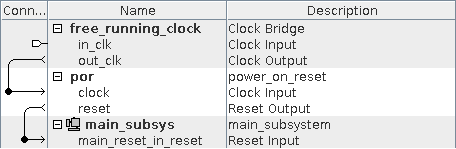
\includegraphics[scale=0.675]{por_qsys}
\caption{POR Qsys System}
\label{fig:por_qsys}
\end{figure}

Please refer to the \emph{por} instance of the \emph{power\_on\_reset} component shown in Figure \ref{fig:por_qsys}.  The POR component requires a free running and stable \emph{clock} input, typically provided by an external clock, not an internal PLL.  When the POR component enters user mode the \emph{reset} output will be asserted and will remain asserted until the user specified clock count occurs.  The reset output from the POR component can be applied to any Qsys reset input interface.  In the example shown above in Figure \ref{fig:por_qsys}, you can see that we simply have this reset drive an entire subsystem reset input interface.

\begin{figure}[H]
\begin{subfigure}{0.495\textwidth}
\centering
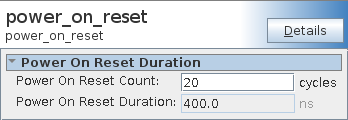
\includegraphics[scale=0.675]{por_parameters}
\caption{POR Parameters}
\label{fig:por_parameters}
\end{subfigure}
\begin{subfigure}{0.495\textwidth}
\centering
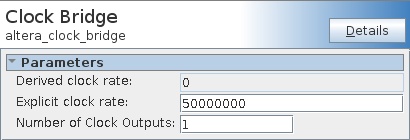
\includegraphics[scale=0.675]{por_clock_parameters}
\caption{Free Running Clock Parameters}
\label{fig:por_clock_parameters}
\end{subfigure}
\caption{Parameters}
\label{fig:por_qsys_parameters}
\end{figure}

The POR component requires one parameter to be set which indicates how long the shift chain is that implements the reset delay.  In the example above you can see that we have set the Power On Reset Count to 20 clock cycles, and the component knows that the frequency that our free running clock has declared is 50MHz so the POR component displays the calculated duration in nanoseconds.

\end{flushleft}

%-------------------------------------------------------------------------------
\section*{Reset Debouncer Component}
% must manually add TOC reference for unnumbered section
\addcontentsline{toc}{section}{Reset Debouncer Component}
%-------------------------------------------------------------------------------
\begin{flushleft}
\noindent
The Reset Debouncer component is designed to debounce noisy reset signals like you may find in a push button switch that generates a reset input to your device.  When an assertion edge is detected at the \emph{reset\_input} interface, the Reset Debouncer will assert the \emph{reset\_output} interface and it will remain asserted until the \emph{reset\_input} signal is deasserted for a user specified amount of time. Then the Reset Debouncer will release the \emph{reset\_output} interface. There is an Avalon slave interface on the Reset Debouncer such that a master in the system can read the internal status register to examine the assertion and deassertion counts experienced by the component.  The \emph{power\_on\_reset} input ensures that the internal counters are cleared only at power on.  For more details on the component functionality please refer to the comment block at the top of the HDL file that describes the component, or see code Listing \ref{ResetDebouncerListing} below.

\begin{figure}[H]
\centering
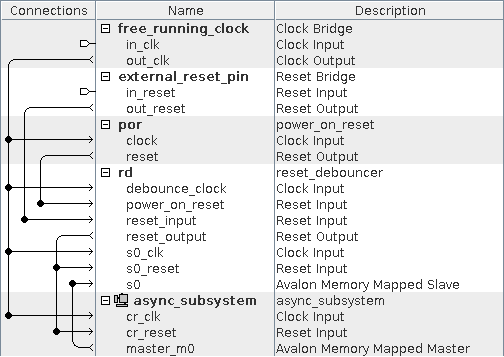
\includegraphics[scale=0.675]{rd_qsys}
\caption{Reset Debouncer Qsys System}
\label{fig:rd_qsys}
\end{figure}

Please refer to the \emph{rd} instance of the \emph{reset\_debouncer} component shown in Figure \ref{fig:rd_qsys}.  The \emph{debounce\_clock} should be driven by a free running and stable clock, typically provided by an external clock, not an internal PLL.  The \emph{power\_on\_reset} input should be driven by a signal as we described in the Power On Reset Component section above.  The \emph{reset\_input} interface should be driven by the potentially noisy reset input signal.  The \emph{reset\_output} interface can drive any appropriate Qsys reset input interface.  The \emph{s0\_clk} and \emph{s0\_reset} should be driven by appropriate clock and reset domains to support the \emph{s0} Avalon slave interface.

\begin{figure}[H]
\centering
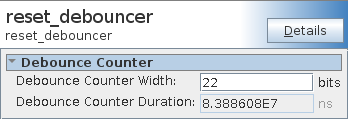
\includegraphics[scale=0.675]{rd_parameters}
\caption{Reset Debouncer Parameters}
\label{fig:rd_parameters}
\end{figure}

The only parameter that this component requires is the width of the debounce counter which determines the terminal count for the debounce delay.  In this example we have set this to 22 bits which produces a terminal count of about 84 milliseconds.

\end{flushleft}

%-------------------------------------------------------------------------------
\section*{Reset Event Counter Component}
% must manually add TOC reference for unnumbered section
\addcontentsline{toc}{section}{Reset Event Counter Component}
%-------------------------------------------------------------------------------
\begin{flushleft}
\noindent
The Reset Event Counter component is designed to count reset events.  When an assertion or deassertion edge is detected at the \emph{reset\_event} interface, the Reset Event Counter will increment the assertion or deassertion counters respectively.  There is an Avalon slave interface on the Reset Event Counter such that a master in the system can read the internal status register to examine the assertion and deassertion events experienced by the component.  The \emph{power\_on\_reset} input ensures that the internal counters are cleared only at power on.  For more details on the component functionality please refer to the comment block at the top of the HDL file that describes the component, or see code Listing \ref{ResetEventCounterListing} below.

\begin{figure}[H]
\centering
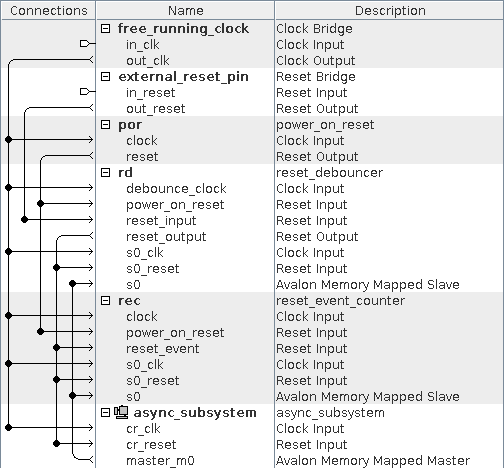
\includegraphics[scale=0.675]{rec_qsys}
\caption{Reset Event Counter Qsys System}
\label{fig:rec_qsys}
\end{figure}

Please refer to the \emph{rec} instance of the \emph{reset\_event\_counter} component shown in Figure \ref{fig:rec_qsys}.  The \emph{clock} input should be driven by a free running and stable clock, typically provided by an external clock, not an internal PLL.  The \emph{power\_on\_reset} input should be driven by a signal as we described in the Power On Reset Component section above.  The \emph{reset\_event} interface should be driven by the Qsys reset output interface that you wish to monitor.  The \emph{s0\_clk} and \emph{s0\_reset} should be driven by appropriate clock and reset domains to support the \emph{s0} Avalon slave interface.

\begin{figure}[H]
\centering
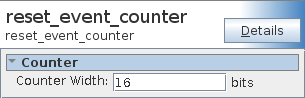
\includegraphics[scale=0.675]{rec_parameters}
\caption{Reset Event Counter Parameters}
\label{fig:rec_parameters}
\end{figure}

The only parameter that this component requires is the width of the counters which determines the limit for the number of events that can be counted.  In this example we have set this to 16 bits which produces a 16 bit assertion counter and a 16 bit deassertion counter.

\end{flushleft}

%-------------------------------------------------------------------------------
\section*{Trivial Default Avalon Slave Component}
% must manually add TOC reference for unnumbered section
\addcontentsline{toc}{section}{Trivial Default Avalon Slave Component}
%-------------------------------------------------------------------------------
\begin{flushleft}
\noindent
The Trivial Default Avalon Slave component is designed to act as a default slave in Qsys systems.  Qsys allows the user to designate particular slaves in the system to decode as the default slave when an otherwise undecoded address is presented to the interconnect fabric.  Each interconnect for a given master may have a default slave designated, so there may be multiple default slaves in any given Qsys system.  For more details on the component functionality please refer to the comment block at the top of the HDL file that describes the component, or see code Listing \ref{TrivalDefaultAvalonSlaveListing} below.

\begin{figure}[H]
\centering
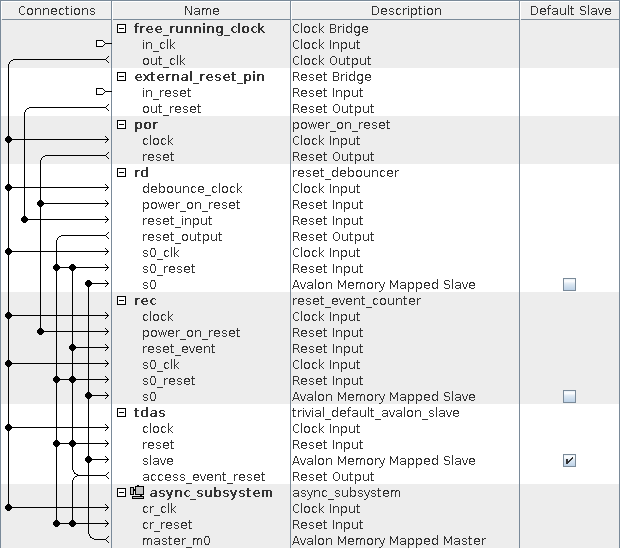
\includegraphics[scale=0.675]{tdas_qsys}
\caption{Trivial Default Avalon Slave Qsys System}
\label{fig:tdas_qsys}
\end{figure}

Please refer to the \emph{tdas} instance of the \emph{trivial\_default\_avalon\_slave} component shown in Figure \ref{fig:tdas_qsys}.  The \emph{clock} and \emph{reset} should be driven by appropriate clock and reset domains to support the \emph{slave} Avalon slave interface.  In this example we have enabled the \emph{access\_event\_reset} interface which can be connected to any Qsys reset input interface that you desire.  The \emph{tdas} slave is designated to be the default slave in this interconnect by the check box in the rightmost \textquote{Default Slave} column.

\begin{figure}[H]
\centering
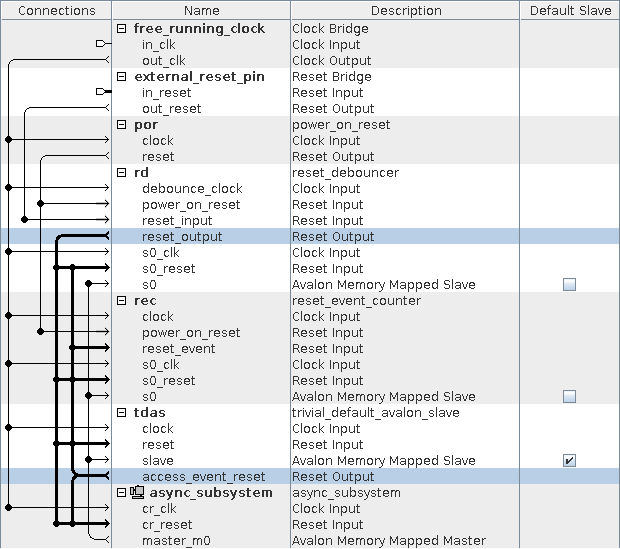
\includegraphics[scale=0.675]{tdas_resets}
\caption{TDAS Example Reset Highlights}
\label{fig:tdas_resets}
\end{figure}

In Figure \ref{fig:tdas_resets} we have highlighted the main system reset sources in the Qsys system.  There is a POR reset and an external reset pin in the example that are not highlighted, but the \emph{reset\_output} of the \emph{rd} component and the \emph{access\_event\_reset} of the \emph{tdas} component are connected to each of the main system reset inputs, which are primarily comprised of Avalon MM interfaces in this system.  You should notice that the \emph{reset\_event} input on the \emph{rec} component is only connected to the \emph{access\_event\_reset} reset output.  This means that the Reset Event Counter will only count resets that are generated by the Trivial Default Avalon Slave component.

\begin{figure}[H]
\centering
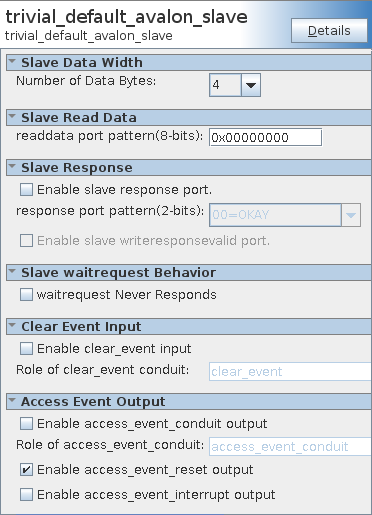
\includegraphics[scale=0.675]{tdas_parameters}
\caption{Trivial Default Avalon Slave Parameters}
\label{fig:tdas_parameters}
\end{figure}

The Trivial Default Avalon Slave component has a number of parameters that you can implement.
\begin{itemize}

\item \texttt{\underline{Number of Data Bytes}} - this parameter allows you to specify how many byte lanes you want the component to expose on the slave interface.  There is no requirement for this to be anything in particular, but you can optimize the interconnect fabric that is generated by Qsys by aligning the size of this slave with the masters that connect to it so that no unnecessary width adapters are generated for instance.

\item \texttt{\underline{readdata port pattern}} - this parameter allows you to specify what data pattern will be returned by the default slave if it responds to a read access.  You may only specify 8-bits here, and those 8-bits are repeated in every byte lane of the slave.  A useful value to program into this is 0x00 when you connect this default slave to a Nios II processor's instruction master.  That way if the Nios II jumps to an undecoded address in the system it will essentially fetch a \textquote{\texttt{call 0x00}} instruction which will force it to jump to address 0x00.  As long as there is no decoded slave peripheral at location 0x00, the default slave will be accessed again and again provide the same instruction to the Nios II.  When developing in the lab this can be a desirable failure mode that allows you to connect to the Nios II processor with a debugger.

\item \texttt{\underline{Enable slave response port}} - this parameter enables the Avalon \emph{response} port which allows you to signal read responses back from the slave.

\item \texttt{\underline{response port pattern}} - this parameter allows you to specify what the read or write response pattern will be if the \emph{response} or \emph{writeresponse} ports are enabled.  There are four options that can be signaled, \emph{OKAY}, \emph{RESERVED}, \emph{SLAVE ERROR} and \emph{DECODE ERROR}.

\item \texttt{\underline{Enable slave writeresponse port}} - this parameter enables the Avalon \emph{writeresponse} port that allows you to signal write responses back from the slave.

\item \texttt{\underline{waitrequest Never Responds}} - this parameter prevents the default slave from ever responding to any read or write accesses.  Any master that reads or writes this slave when this mode is enabled will stall forever.  This state can only be cleared by asserting the \emph{reset} to the component, or asserting the \emph{clear\_event} signal if that interface has been enabled.

\item \texttt{\underline{Enable clear\_event input}} - this parameter enables the \emph{clear\_event} conduit interface which allows you to clear any access events that have been captured by this component.

\item \texttt{\underline{Role of clear\_event conduit}} - this parameter sets the role of the \emph{clear\_event} conduit signal.  This allows you to connect this conduit directly to another conduit interface within Qsys.

\item \texttt{\underline{Enable access\_event\_conduit output}} - this parameter exposes the \emph{access\_event\_conduit} interface which is asserted whenever a read or write transaction is received at the default slave.  You can clear this event by resetting the component or asserting the \emph{clear\_event} conduit input.

\item \texttt{\underline{Role of access\_event\_conduit}} - this parameter sets the role of the \emph{access\_event\_conduit} conduit signal.  This allows you to connect this conduit directly to another conduit interface within Qsys.

\item \texttt{\underline{Enable access\_event\_reset output}} - this parameter exposes the \emph{access\_event\_reset} interface which is asserted whenever a read or write transaction is received at the default slave.  You can clear this reset by resetting the component or asserting the \emph{clear\_event} conduit input.

\item \texttt{\underline{Enable access\_event\_interrupt output}} - this parameter exposes the \emph{access\_event\_interrupt} interface which is asserted whenever a read or write transaction is received at the default slave.  You can clear this interrupt by resetting the component or asserting the \emph{clear\_event} conduit input.

\end{itemize}

\end{flushleft}

%-------------------------------------------------------------------------------
\section*{PLL Reset Monitor Component}
% must manually add TOC reference for unnumbered section
\addcontentsline{toc}{section}{PLL Reset Monitor Component}
%-------------------------------------------------------------------------------
\begin{flushleft}
\noindent
The PLL Reset Monitor component is designed to reset and monitor the locked state of an Altera PLL.
\newline
\newline
PLL maintenance can be a bit tedious, a PLL can stutter into the locked state, and once locked it may drop out of lock for only a brief instance which requires the PLL to be reset to recover.  All PLLs should be reset as the FPGA enters user mode to ensure that the desired PLL configuration is properly achieved as the PLL attempts its initial lock.  After you release reset to the PLL you must allow the PLL to potentially stutter in and out of the locked state for the minimum lock period which is generally defined as 1ms for most Altera PLLs.  This means that you should ignore lock assertions during this initial lock period as you may see false lock assertions.  Some later generation FPGA families are equipped with internal hysteresis that masks the locked output for about 1K cycles of the reference clock, but even then you could witness stuttering in certain situations.  Once the initial lock period has expired if the locked output ever deasserts at all, even for a nanosecond, then you must assume that the PLL has lost lock and you must reset the PLL in order to ensure that it reacquires the desired PLL configuration again.
\newline
\newline
Now in reality, with a properly designed circuit board, power supplies and filtering, and no assembly defects, the behavior of the Altera PLL is generally much more stable and reliable than the previous paragraph may indicate.  Most folks never witness any lock stuttering as the PLL exits reset, nor do they ever witness PLL lock failures after lock has been achieved, especially at room temperature in a well controlled lab environment.  And it is possible that you can characterize the device to behave within much better tolerances in your specific environmental conditions.  Nevertheless, the conditions described above must be considered as worst case possibilities, and you may witness this behavior if anything about your design or assembly or deployment environment are marginal in any way.
\newline
\newline
The PLL Reset Monitor component attempts to satisfy all of these maintenance requirements for a PLL. The component provides the user with a \emph{pll\_reset\_request} input that you assert when you wish to reset the PLL.  The component then asserts \emph{pll\_reset} to the PLL for a user specified duration.  Most Altera PLLs require only a 10ns reset pulse to ensure the reset is captured internally. When the component releases \emph{pll\_reset} it then monitors the \emph{pll\_locked} input to determine if the PLL has gained lock and maintains lock.  If the user specified lock wait time expires and the PLL is locked, then the \emph{lock\_success\_reset} output is asserted, and from that point forward if the PLL ever looses lock, then the \emph{lock\_failure\_reset} output is asserted.  The component also provides an Avalon slave interface so that masters in the Qsys system can examine the status register inside the component.  By connecting these signals appropriately in your Qsys system, you should be able to achieve most common reset responses required in environments that manage PLLs.  For more details on the component functionality please refer to the comment block at the top of the HDL file that describes the component, or see code Listing \ref{PLLResetMonitorListing} below.

\begin{figure}[H]
\centering
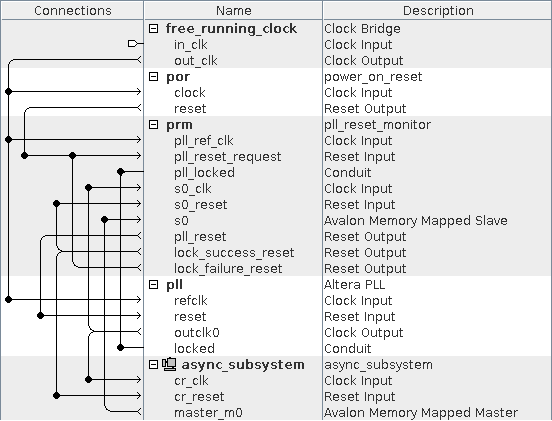
\includegraphics[scale=0.675]{prm_qsys}
\caption{PLL Reset Monitor Qsys System}
\label{fig:prm_qsys}
\end{figure}

Please refer to the \emph{prm} instance of the \emph{pll\_reset\_monitor} component shown in Figure \ref{fig:prm_qsys}.  The \emph{pll\_ref\_clock} should be driven by a free running and stable clock, just like the actual PLL reference clock.  This is typically provided by an external clock, not an internal PLL.  The \emph{s0\_clk} and \emph{s0\_reset} should be driven by appropriate clock and reset domains to support the \emph{s0} Avalon slave interface.  The other signals on this component will be highlighted and described below.

\begin{figure}[H]
\centering
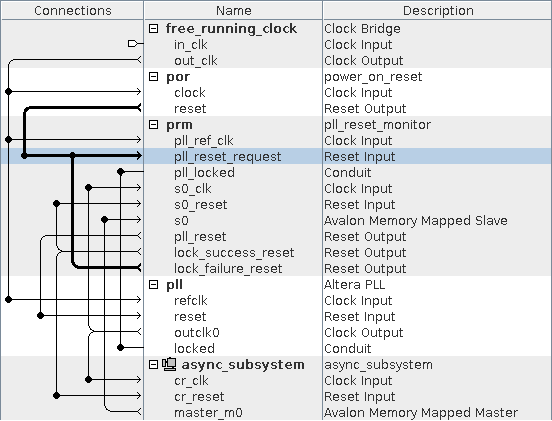
\includegraphics[scale=0.675]{prm_pll_reset_request}
\caption{PRM Reset Request Highlight}
\label{fig:prm_pll_reset_request}
\end{figure}

In Figure \ref{fig:prm_pll_reset_request} we have highlighted the \emph{pll\_reset\_request} input.  You can see that it is driven by the POR reset output and the \emph{lock\_failure\_reset} output.  The POR reset ensures that this component resets the PLL as the FPGA enters user mode, and the \emph{lock\_failure\_reset} will reset the PLL if a lock failure is ever detected.

\begin{figure}[H]
\centering
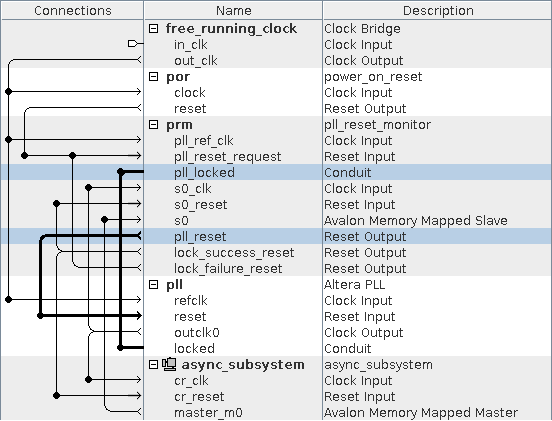
\includegraphics[scale=0.675]{prm_pll_reset}
\caption{PRM PLL Reset Highlight}
\label{fig:prm_pll_reset}
\end{figure}

In Figure \ref{fig:prm_pll_reset} we have highlighted the \emph{pll\_reset} output.  You can see that it drives the PLL reset input.  The \emph{pll\_locked} input is also highlighted, it receives the locked indication from the PLL so that the PLL Reset Monitor component can monitor the lock status of the PLL and respond accordingly.

\begin{figure}[H]
\centering
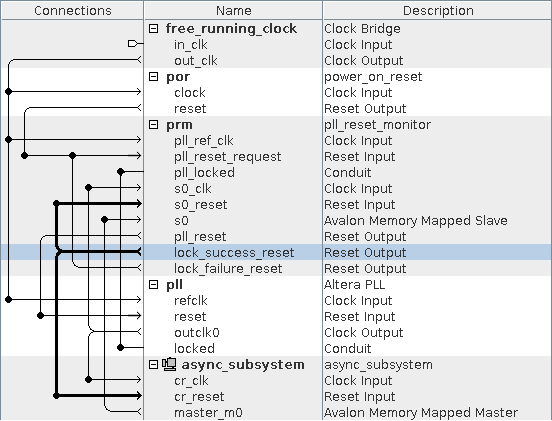
\includegraphics[scale=0.675]{prm_pll_lock_success_reset}
\caption{PRM Lock Success Reset Highlight}
\label{fig:prm_pll_lock_success_reset}
\end{figure}

In Figure \ref{fig:prm_pll_lock_success_reset} we have highlighted the \emph{lock\_success\_reset} output.  You can see that it drives all of the basic Qsys system resets, primarily involving the Avalon MM interfaces.  When the PLL Reset Monitor component is reset, this \emph{lock\_success\_reset} output will be driven low, and when the PLL successfully achieves locked status, this output will be driven high.  As you'll see in the next figure, we can instruct Qsys how to interpret the polarity of this as a reset interface, so we can easily configure this reset to hold the main Qsys system elements in reset until the PLL has achieved lock.

\begin{figure}[H]
\centering
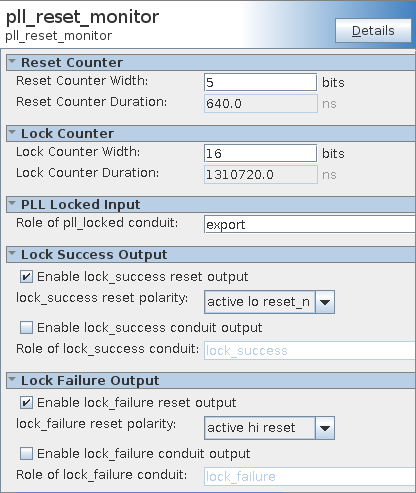
\includegraphics[scale=0.675]{prm_parameters}
\caption{PLL Reset Monitor Parameters}
\label{fig:prm_parameters}
\end{figure}

The PLL Reset Monitor component has a number of parameters that you can implement.
\begin{itemize}

\item \texttt{\underline{Reset Counter Width}} - this parameter allows you to specify the width of the PLL reset duration counter.  This will be the duration of the reset pulse that the component delivers to the PLL.  If the frequency of the \emph{pll\_ref\_clk} is known, then this component will also calculate the duration of the PLL reset pulse in nanoseconds for you.

\item \texttt{\underline{Lock Counter Width}} - this parameter allows you to specify the width of the PLL lock mask counter.  This will be the duration that the component masks or ignores lock stutter after it releases the PLL reset output.  If the frequency of the \emph{pll\_ref\_clk} is known, then this component will also calculate the duration of the PLL lock mask duration in nanoseconds for you.

\item \texttt{\underline{Role of pll\_locked conduit}} - this parameter sets the role of the \emph{pll\_locked} conduit signal.  This should allow you to align the role of this conduit interface with the role of the locked conduit from the PLL so that you can connect the two conduits within the Qsys system.

\item \texttt{\underline{Enable lock\_success reset output}} - this parameter exposes the lock success indication as a reset interface so that you can connect this to other reset interfaces within the Qsys system.

\item \texttt{\underline{lock\_success reset polarity}} - this parameter sets the polarity of the lock success reset interface.  This does not change the behavior of the \emph{lock\_success\_reset} output, it simply changes the way Qsys interprets the signal as either an active high \textquote{\texttt{reset}} interface or as an active low \textquote{\texttt{reset\_n}} interface.  When this component is reset, this interface will drive low and when PLL lock is successfully achieved, this interface will drive high, regardless of how this parameter is set.

\item \texttt{\underline{Enable lock\_success conduit output}} - this parameter exposes the lock success indication as a conduit interface so that you can connect this to other conduit interfaces within the Qsys system.

\item \texttt{\underline{Role of lock\_success conduit}} - this parameter sets the role of the lock success conduit signal.  This allows you to connect this conduit directly to another conduit interface within Qsys.

\item \texttt{\underline{Enable lock\_failure reset output}} - this parameter exposes the lock failure indication as a reset interface so that you can connect this to other reset interfaces within the Qsys system.

\item \texttt{\underline{lock\_failure reset polarity}} - this parameter sets the polarity of the lock failure reset interface.  This does not change the behavior of the \emph{lock\_failure\_reset} output, it simply changes the way Qsys interprets the signal as either an active high \textquote{\texttt{reset}} interface or as an active low \textquote{\texttt{reset\_n}} interface.  When this component is reset, this interface will drive low and when a PLL lock failure is detected, this interface will drive high, regardless of how this parameter is set.

\item \texttt{\underline{Enable lock\_failure conduit output}} - this parameter exposes the lock failure indication as a conduit interface so that you can connect this to other conduit interfaces within the Qsys system.

\item \texttt{\underline{Role of lock\_failure conduit}} - this parameter sets the role of the lock failure conduit signal.  This allows you to connect this conduit directly to another conduit interface within Qsys.

\end{itemize}

\end{flushleft}

%-------------------------------------------------------------------------------
\section*{Reset Assertion Delay Component}
% must manually add TOC reference for unnumbered section
\addcontentsline{toc}{section}{Reset Assertion Delay Component}
%-------------------------------------------------------------------------------
\begin{flushleft}
\noindent
The Reset Assertion Delay component is designed to implement a user specified delay between two reset output interfaces.  The first reset output is asserted immediately as this component detects a reset input event, and the delayed reset output is asserted at some user specified delay later.  This is useful in situations where you may need to reset a PLL for instance but you need to place other system logic into reset before you reset the PLL.  This can arise in situations where you may have synchronous reset domains, or other situations that cannot tolerate the loss of a clock during the PLL reset event.  Most Altera PLLs will disable the clock outputs while they are in the reset state.  For more details on the component functionality please refer to the comment block at the top of the HDL file that describes the component, or see code Listing \ref{ResetAssertionDelayListing} below.

\begin{figure}[H]
\centering
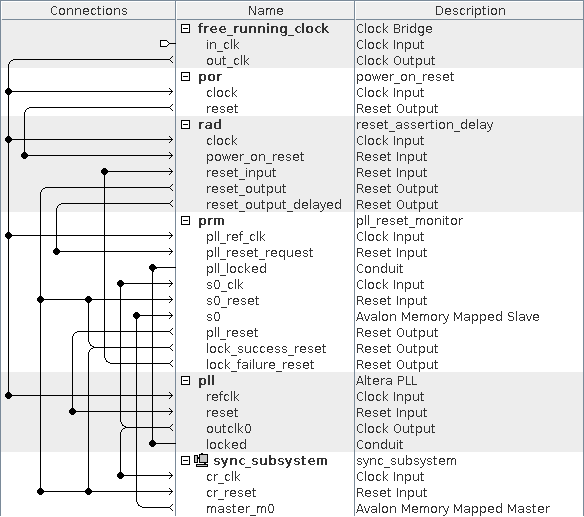
\includegraphics[scale=0.675]{rad_qsys}
\caption{Reset Assertion Delay Qsys System}
\label{fig:rad_qsys}
\end{figure}

Please refer to the \emph{rad} instance of the \emph{reset\_assertion\_delay} component shown in Figure \ref{fig:rad_qsys}.  The \emph{clock} should be driven by a free running and stable clock, typically provided by an external clock, not an internal PLL.  The other signals on this component will be highlighted and described below.

\begin{figure}[H]
\centering
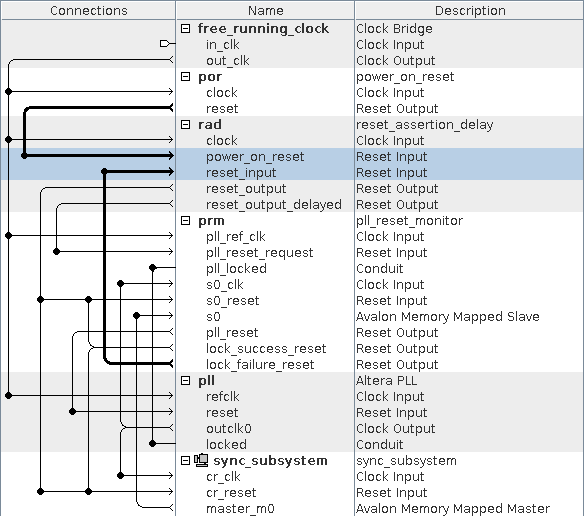
\includegraphics[scale=0.675]{rad_reset_inputs}
\caption{RAD Reset Inputs Highlight}
\label{fig:rad_reset_inputs}
\end{figure}

In Figure \ref{fig:rad_reset_inputs} we have highlighted the \emph{power\_on\_reset} input and the \emph{reset\_input} ports.  You can see that these are driven by the POR reset output and the \emph{lock\_failure\_reset} output from the PLL Reset Monitor that we described above.  The POR reset ensures that this component asserts both reset outputs as the FPGA enters user mode, and the \emph{lock\_failure\_reset} will trigger the reset assertion delay sequence if a lock failure is ever detected.

\begin{figure}[H]
\centering
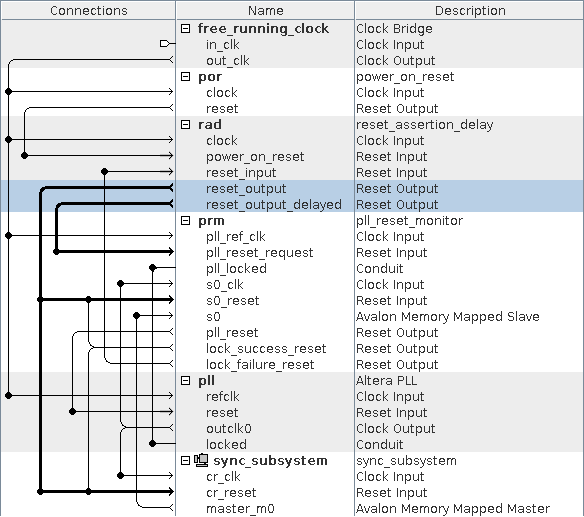
\includegraphics[scale=0.675]{rad_reset_outputs}
\caption{RAD Reset Outputs Highlight}
\label{fig:rad_reset_outputs}
\end{figure}

In Figure \ref{fig:rad_reset_outputs} we have highlighted the \emph{reset\_output} and \emph{reset\_output\_delayed} outputs.  You can see that the \emph{reset\_output} signal drives the reset inputs of the main system components that we want to place into reset prior to resetting the PLL.  And the \emph{reset\_output\_delayed} signal drives the PLL Reset Monitor \emph{pll\_reset\_request} input to reset the PLL.
\newline
\newline
Please note that in this Reset Assertion Delay Qsys system we have changed the main subsystem name shown at the bottom of the image from \emph{async\_subsystem} as it has been named in all of the previous component example systems to \emph{sync\_subsystem}.  This is intended to imply that the reset requirements inside that Qsys subsystem are synchronous rather than asynchronous.  You can easily create this reset requirement in a Qsys system by simply inserting an OnChip Memory component, as those components require synchronous resets.  You can identify Qsys components that require synchronous resets by the presence of the \emph{reset\_req} Avalon port on the reset interface.

\begin{figure}[H]
\centering
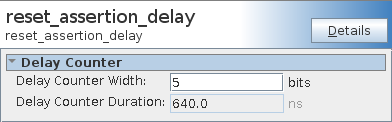
\includegraphics[scale=0.675]{rad_parameters}
\caption{Reset Assertion Delay Parameters}
\label{fig:rad_parameters}
\end{figure}

The PLL Reset Monitor component has one parameter that you specify, the delay counter width.  This sets the duration of the delay between the assertion from the \emph{reset\_output} signal to the \emph{reset\_output\_delayed} signal.  If the frequency of the \emph{clock} is known, then this component will also calculate the duration of the delay in nanoseconds for you.

\end{flushleft}

%-------------------------------------------------------------------------------
\section*{Event Timer Component}
% must manually add TOC reference for unnumbered section
\addcontentsline{toc}{section}{Event Timer Component}
%-------------------------------------------------------------------------------
\begin{flushleft}
\noindent
The Event Timer component is designed to provide more complex sequencing of system resets that may require a delay to allow for certain logic blocks to initialize or calibrate themselves before moving along with the system reset sequencing requirements.  This situation can arise in Qsys systems that implement EMIF controllers where there is an integrated PLL which must be managed and the controller logic goes through a calibration phase and an initialization phase before the controller is ready for use.  In the example EMIF system that we show below, we assume that the user wants to hold off the main system reset release until the EMIF controller has achieved PLL lock, successfully calibrated and then successfully initialized itself.  To accomplish this we implement two Event Timer components, one that monitors the calibration status and one that monitors the initialization status.  Fundamentally what the Event Timer component does is monitor the state of an event input to detect if the event has asserted within a user specified period of time otherwise a timeout condition occurs and a timeout output indication asserts.  If the event input asserts within the timeout period then an acquired output indication asserts and the event input is further monitored in case it ever deasserts.  If the event input deasserts after a successful assertion, then a loss output indication asserts.  For more details on the component functionality please refer to the comment block at the top of the HDL file that describes the component, or see code Listing \ref{EventTimerListing} below.

\begin{figure}[H]
\centering
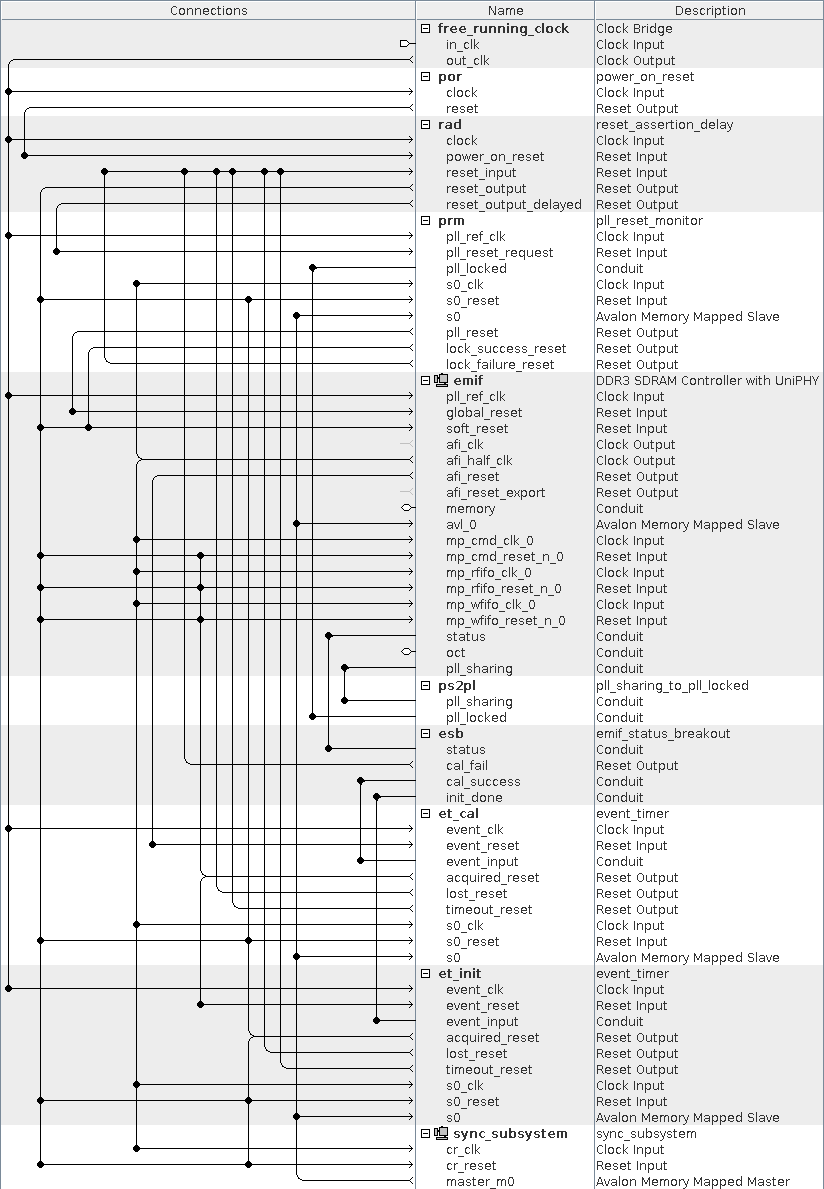
\includegraphics[scale=0.675]{emif_qsys}
\caption{Event Timer Qsys System}
\label{fig:emif_qsys}
\end{figure}

Please refer to the \emph{et\_cal} instance of the \emph{event\_timer} component shown in Figure \ref{fig:emif_qsys}.  The \emph{event\_clk} should be driven by a free running and stable clock, typically provided by an external clock, not an internal PLL.  The \emph{event\_reset} should be driven by an appropriate reset output, typically driven by an appropriate stage of the overall system reset sequencing logic.  The Event Timer component can only be cleared or restarted by a reset on the \emph{event\_reset} port. The \emph{acquired\_reset}, \emph{lost\_reset} and \emph{timeout\_reset} are the outputs that represent the event acquisition state, event lost state and the event timeout state respectively.  These outputs should be wired into the Qsys system to affect the desired sequencing.  A more detailed discussion of the reset sequencing strategy in this example will be shown below.  The \emph{s0\_clk} and \emph{s0\_reset} should be driven by appropriate clock and reset domains to support the \emph{s0} Avalon slave interface.  The Avalon slave interface allows masters in the system to query the status register in the component.

\begin{figure}[H]
\centering
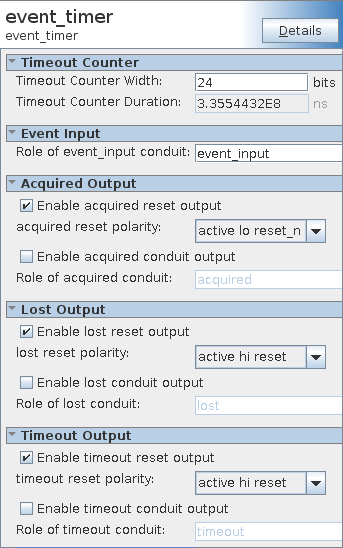
\includegraphics[scale=0.675]{et_parameters}
\caption{Event Timer Parameters}
\label{fig:et_parameters}
\end{figure}

The Event Timer component has a number of parameters that you can implement.
\begin{itemize}

\item \texttt{\underline{Timeout Counter Width}} - this parameter allows you to specify the width of the timeout duration counter.  This will be the duration that the component waits after it exits the reset state before it declares a timeout condition.  If the frequency of the \emph{event\_clk} is known, then this component will also calculate the duration of the delay in nanoseconds for you.

\item \texttt{\underline{Role of event\_input conduit}} - this parameter sets the role of the \emph{event\_input} conduit signal.  This allows you to connect this conduit directly to another conduit interface within Qsys.

\item \texttt{\underline{Enable acquired reset output}} - this parameter exposes the acquired indication as a reset interface so that you can connect this to other reset interfaces within the Qsys system.

\item \texttt{\underline{acquired reset polarity}} - this parameter sets the polarity of the acquired reset interface.  This does not change the behavior of the \emph{acquired\_reset} output, it simply changes the way Qsys interprets the signal as either an active high \textquote{\texttt{reset}} interface or as an active low \textquote{\texttt{reset\_n}} interface.  When this component is reset, this interface will drive low and when the acquired state is achieved, this interface will drive high, regardless of how this parameter is set.

\item \texttt{\underline{Enable acquired conduit output}} - this parameter exposes the acquired indication as a conduit interface so that you can connect this to other conduit interfaces within the Qsys system.

\item \texttt{\underline{Role of acquired conduit}} - this parameter sets the role of the acquired conduit signal.  This allows you to connect this conduit directly to another conduit interface within Qsys.

\item \texttt{\underline{Enable lost reset output}} - this parameter exposes the lost indication as a reset interface so that you can connect this to other reset interfaces within the Qsys system.

\item \texttt{\underline{lost reset polarity}} - this parameter sets the polarity of the lost reset interface.  This does not change the behavior of the \emph{lost\_reset} output, it simply changes the way Qsys interprets the signal as either an active high \textquote{\texttt{reset}} interface or as an active low \textquote{\texttt{reset\_n}} interface.  When this component is reset, this interface will drive low and when the lost state is achieved, this interface will drive high, regardless of how this parameter is set.

\item \texttt{\underline{Enable lost conduit output}} - this parameter exposes the lost indication as a conduit interface so that you can connect this to other conduit interfaces within the Qsys system.

\item \texttt{\underline{Role of lost conduit}} - this parameter sets the role of the lost conduit signal.  This allows you to connect this conduit directly to another conduit interface within Qsys.

\item \texttt{\underline{Enable timeout reset output}} - this parameter exposes the timeout indication as a reset interface so that you can connect this to other reset interfaces within the Qsys system.

\item \texttt{\underline{timeout reset polarity}} - this parameter sets the polarity of the timeout reset interface.  This does not change the behavior of the \emph{timeout\_reset} output, it simply changes the way Qsys interprets the signal as either an active high \textquote{\texttt{reset}} interface or as an active low \textquote{\texttt{reset\_n}} interface.  When this component is reset, this interface will drive low and when the timeout state is achieved, this interface will drive high, regardless of how this parameter is set.

\item \texttt{\underline{Enable timeout conduit output}} - this parameter exposes the timeout indication as a conduit interface so that you can connect this to other conduit interfaces within the Qsys system.

\item \texttt{\underline{Role of timeout conduit}} - this parameter sets the role of the timeout conduit signal.  This allows you to connect this conduit directly to another conduit interface within Qsys.

\end{itemize}

\end{flushleft}

%-------------------------------------------------------------------------------
\subsection*{EMIF System Example Explanation}
% must manually add TOC reference for unnumbered section
\addcontentsline{toc}{subsection}{EMIF System Example Explanation}
%-------------------------------------------------------------------------------
\begin{flushleft}
\noindent
Now let's take a deeper look at the architecture presented in the EMIF example from Figure \ref{fig:emif_qsys}.  This system leverages most of the components that have been described above in this HOWTO document.  For more information on any of these supplemental reset components please refer to the appropriate section of this document.

\begin{figure}[H]
\centering
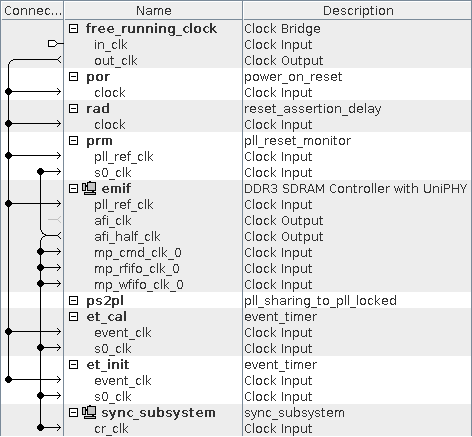
\includegraphics[scale=0.675]{emif_clocks}
\caption{EMIF System Clocks}
\label{fig:emif_clocks}
\end{figure}

In Figure \ref{fig:emif_clocks} we filtered the view to show only the two clock domains in the system.  The free running input clock is driving all of the reset sequencing components and the EMIF PLL reference input.  The \emph{afi\_half\_clk} output from the \emph{emif} instance is driving the rest of the clock inputs in the system.

\begin{figure}[H]
\centering
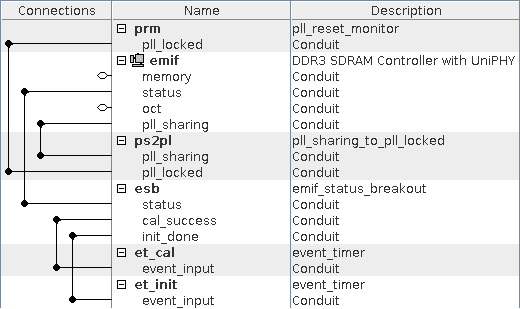
\includegraphics[scale=0.675]{emif_conduits}
\caption{EMIF Conduits}
\label{fig:emif_conduits}
\end{figure}

In Figure \ref{fig:emif_conduits} we filtered the view to show only the conduit interfaces in the system.  There are a couple of useful conduit adapters that are distributed in the Supplemental Reset Components for Qsys project, the \emph{ps2pl} and \emph{esb} instances.  The \emph{ps2pl} component is designed to extract the PLL locked conduit out of the \emph{pll\_sharing} conduit on the EMIF component so that we can feed this into the PLL Reset Monitor component.  The \emph{esb} component is designed to extract the calibration success and initialization done conduits from the \emph{status} conduit on the EMIF component so that we can feed these into the Event Timer components that will monitor these events in our reset sequencing architecture.

\begin{figure}[H]
\centering
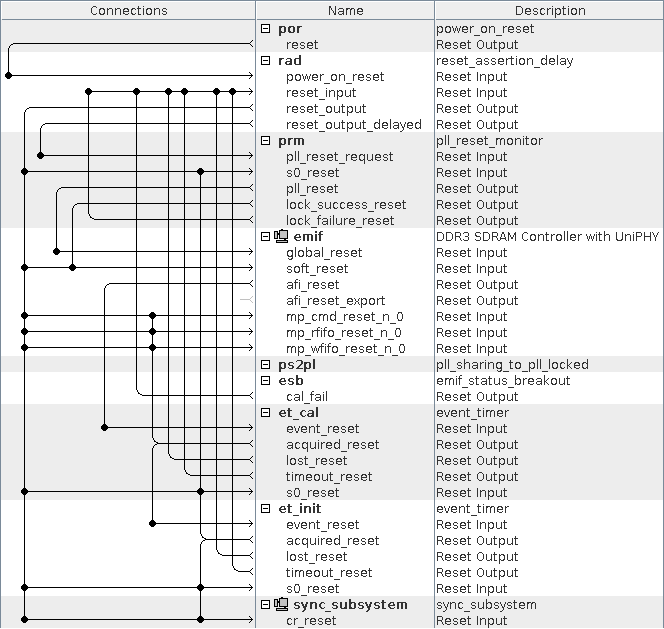
\includegraphics[scale=0.675]{emif_resets}
\caption{EMIF Resets}
\label{fig:emif_resets}
\end{figure}

In Figure \ref{fig:emif_resets} we filtered the view to show only the reset interfaces in the system.  The sequencing of the reset domains begins at the top of this figure and proceeds down to the bottom.  The following figures will highlight each stage of the reset sequence.

\begin{figure}[H]
\centering
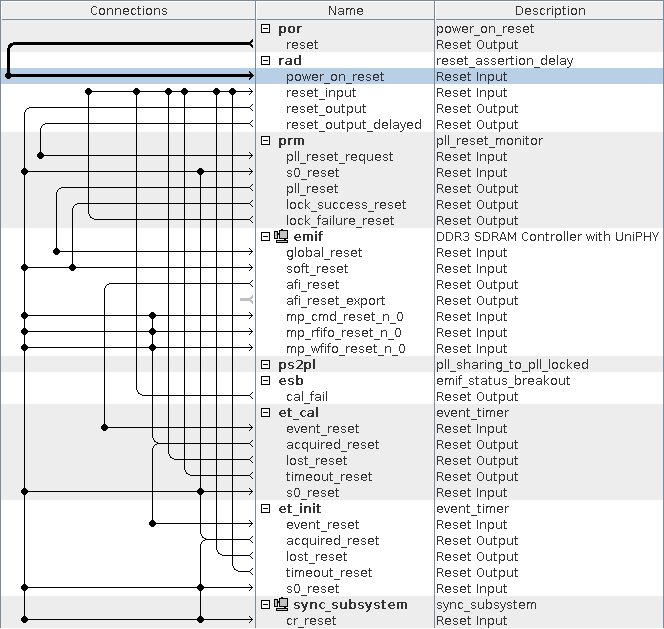
\includegraphics[scale=0.675]{emif_reset_stage_1}
\caption{EMIF Reset Stage 1}
\label{fig:emif_reset_stage_1}
\end{figure}

In Figure \ref{fig:emif_reset_stage_1} we highlight the POR reset that ensures that the Reset Assertion Delay component is reset as the FPGA enters user mode. The outputs of the Reset Assertion Delay component will place everything else in the system into reset.

\begin{figure}[H]
\centering
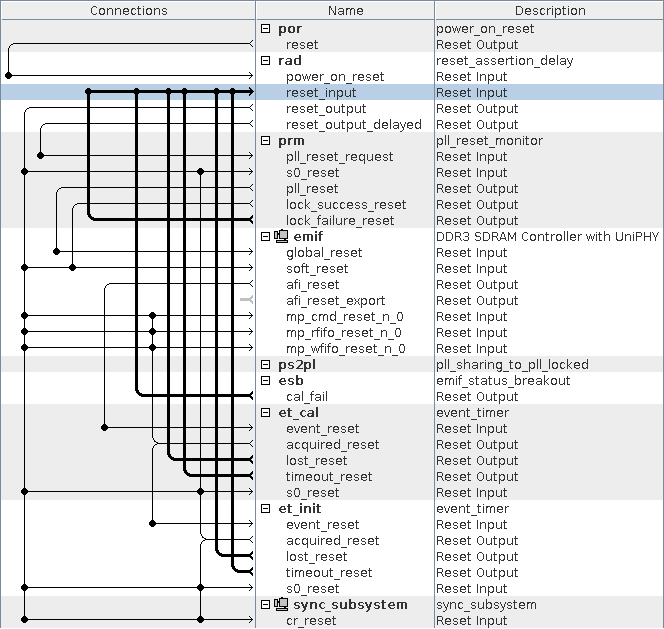
\includegraphics[scale=0.675]{emif_reset_stage_2}
\caption{EMIF Reset Stage 2}
\label{fig:emif_reset_stage_2}
\end{figure}

In Figure \ref{fig:emif_reset_stage_2} we highlight the \emph{reset\_input} of the Reset Assertion Delay component.  This can be considered the main reset for the system, any of the six reset sources that drive this interface can force a complete system reset sequence to occur.  When this reset is asserted the outputs of the Reset Assertion Delay component will place everything else in the system into reset.  The six sources that can cause the complete system reset are as follow:

\begin{itemize}
\item \emph{prm/lock\_failure\_reset} - the lock failure indicator from the PLL Reset Monitor component will trigger the complete system reset when a PLL lock failure is detected in the EMIF PLL.

\item \emph{esb/cal\_fail} - the EMIF calibration failure indicator from the EMIF component will trigger the complete system reset when an EMIF calibration failure is signaled.

\item \emph{et\_cal/lost\_reset} - the EMIF calibration loss indicator from the EMIF calibration Event Timer will trigger the complete system reset when an EMIF calibration success indication is negated.

\item \emph{et\_cal/timeout\_reset} - the EMIF calibration timeout indicator from the EMIF calibration Event Timer will trigger the complete system reset when an EMIF calibration success is not achieved within the specified timeout period.

\item \emph{et\_init/lost\_reset} - the EMIF initialization loss indicator from the EMIF initialization Event Timer will trigger the complete system reset when an EMIF initialization success indication is negated.

\item \emph{et\_init/timeout\_reset} - the EMIF initialization timeout indicator from the EMIF initialization Event Timer will trigger the complete system reset when an EMIF initialization success is not achieved within the specified timeout period.

\end{itemize}

\begin{figure}[H]
\centering
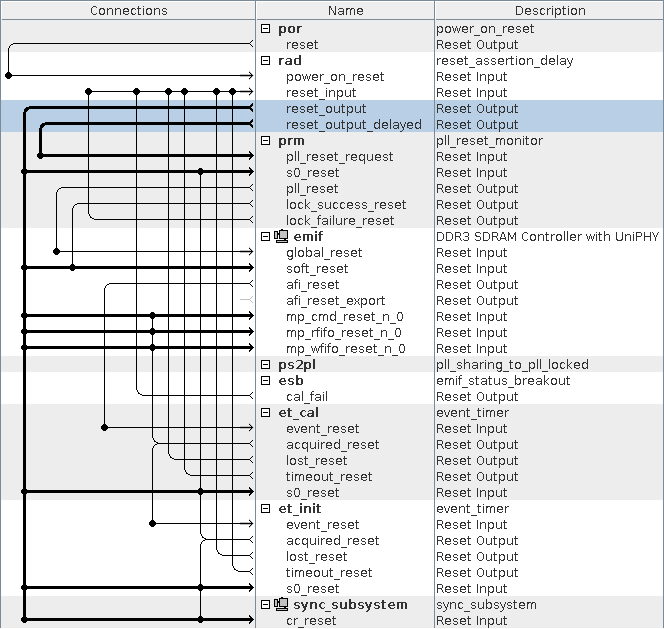
\includegraphics[scale=0.675]{emif_reset_stage_3}
\caption{EMIF Reset Stage 3}
\label{fig:emif_reset_stage_3}
\end{figure}

In Figure \ref{fig:emif_reset_stage_3} we highlight the \emph{reset\_output} interface of the Reset Assertion Delay component which will be asserted immediately when the \emph{reset\_input} interface is driven active and will place all of the main system level resets into reset ahead of the PLL reset.  The \emph{reset\_output\_delayed} interface of the Reset Assertion Delay component is also highlighted.  This reset will be asserted after the user specified delay has passed after the \emph{reset\_output} assertion, and this interface will reset the PLL by driving the PLL Reset Monitor component.

\begin{figure}[H]
\centering
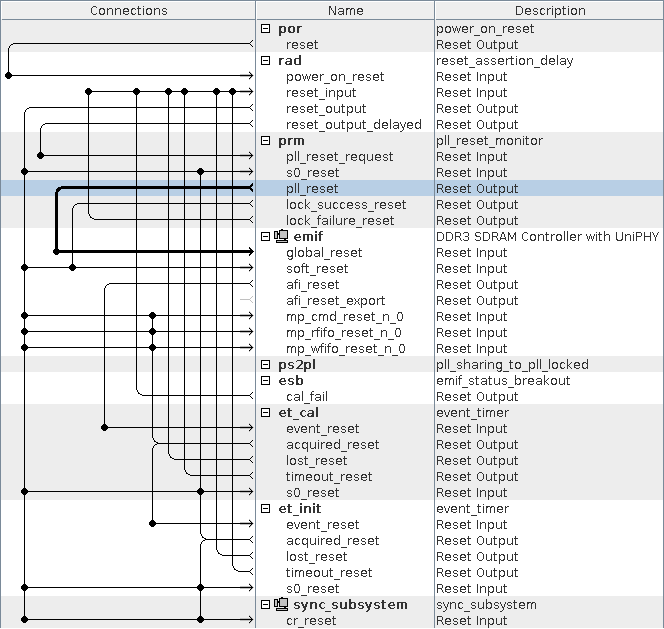
\includegraphics[scale=0.675]{emif_reset_stage_4}
\caption{EMIF Reset Stage 4}
\label{fig:emif_reset_stage_4}
\end{figure}

In Figure \ref{fig:emif_reset_stage_4} we highlight the \emph{pll\_reset} interface of the PLL Reset Monitor component.  This resets the PLL in the EMIF component through the \emph{global\_reset} interface.

\begin{figure}[H]
\centering
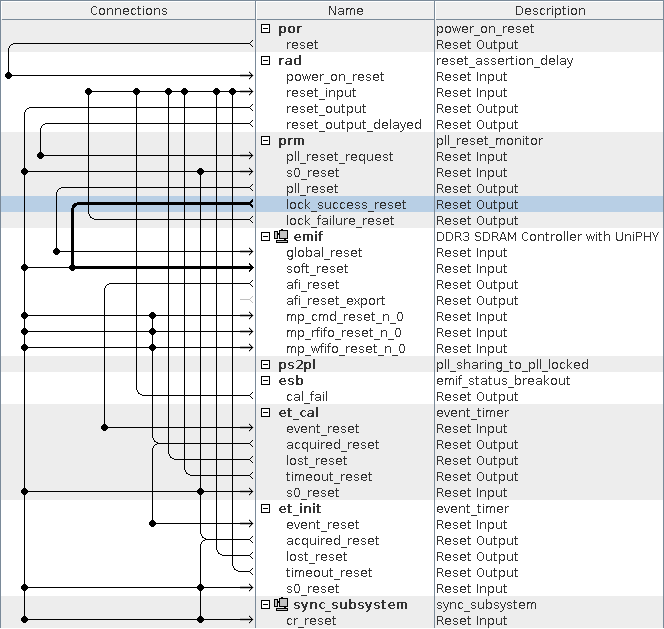
\includegraphics[scale=0.675]{emif_reset_stage_5}
\caption{EMIF Reset Stage 5}
\label{fig:emif_reset_stage_5}
\end{figure}

In Figure \ref{fig:emif_reset_stage_5} we highlight the \emph{lock\_success\_reset} interface of the PLL Reset Monitor component.  After the PLL has been reset, we would expect that it will eventually achieve lock.  Once the PLL lock is achieved, then this reset output will release the \emph{soft\_reset} interface on the EMIF component which allows the EMIF controller to begin it's calibration phase.

\begin{figure}[H]
\centering
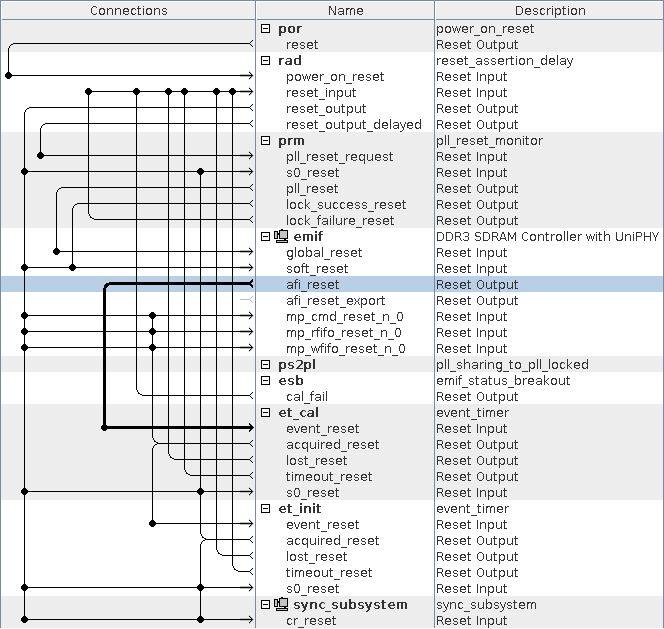
\includegraphics[scale=0.675]{emif_reset_stage_6}
\caption{EMIF Reset Stage 6}
\label{fig:emif_reset_stage_6}
\end{figure}

In Figure \ref{fig:emif_reset_stage_6} we highlight the \emph{afi\_reset} interface of the EMIF component.  This reset will release immediately once there is no reset assertions on the \emph{global\_reset} interface or the \emph{soft\_reset} interface.  When this reset releases it allows the \emph{et\_cal} Event Timer component to begin timing the calibration sequence.

\begin{figure}[H]
\centering
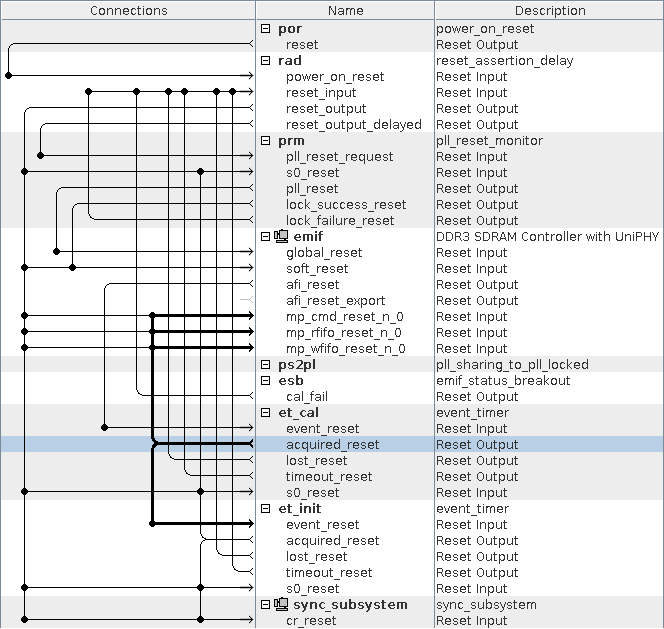
\includegraphics[scale=0.675]{emif_reset_stage_7}
\caption{EMIF Reset Stage 7}
\label{fig:emif_reset_stage_7}
\end{figure}

In Figure \ref{fig:emif_reset_stage_7} we highlight the \emph{acquired\_reset} interface of the EMIF calibration Event Timer component.  When the EMIF calibration indication is successfully captured within the timeout period, this reset will release the \emph{mp\_*fifo\_reset\_n\_0} interfaces on the EMIF component which allows the EMIF to enter its initialization phase.  At the same time the \emph{et\_init} Event Timer component is released and can begin timing the initialization sequence.

\begin{figure}[H]
\centering
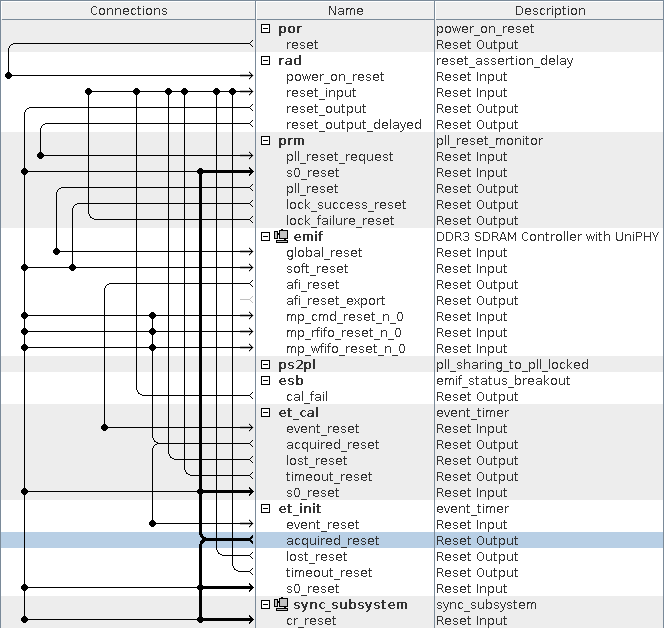
\includegraphics[scale=0.675]{emif_reset_stage_8}
\caption{EMIF Reset Stage 8}
\label{fig:emif_reset_stage_8}
\end{figure}

In Figure \ref{fig:emif_reset_stage_8} we highlight the \emph{acquired\_reset} interface of the EMIF initialization Event Timer component.  When the EMIF initialization indication is successfully captured within the timeout period, this reset will release the system wide reset domain that covers all the Avalon MM interfaces and the \emph{sync\_subsystem}.  At this point, our entire system has sequenced out of reset and it will run uninterrupted unless one of the six system reset request events occur that drive the \emph{reset\_input} of the Reset Assertion Delay component.

\end{flushleft}

%-------------------------------------------------------------------------------
\section*{Reset Until Ack Component}
% must manually add TOC reference for unnumbered section
\addcontentsline{toc}{section}{Reset Until Ack Component}
%-------------------------------------------------------------------------------
\begin{flushleft}
\noindent
The RUA (Reset Until Ack) component is a very trivial component that is intended to assert a reset output signal when a reset assert input signal is active, then hold the reset output asserted until the reset assert input signal is inactive and the reset release input signal is active.  Fundamentally it operates like a simple latch.  For more details on the component functionality please refer to the comment block at the top of the HDL file that describes the component, or see code Listing \ref{ResetUntilAckListing} below.

\begin{figure}[H]
\centering
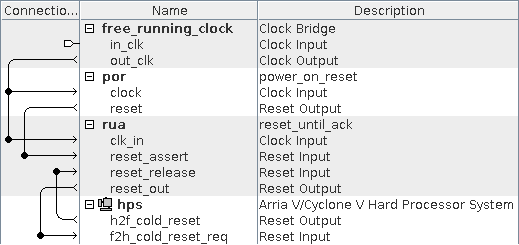
\includegraphics[scale=0.675]{rua_qsys}
\caption{RUA Qsys System}
\label{fig:rua_qsys}
\end{figure}

Please refer to the \emph{rua} instance of the \emph{reset\_until\_ack} component shown in Figure \ref{fig:rua_qsys}.  The RUA component requires a free running and stable \emph{clk\_in} input, typically provided by an external clock, not an internal PLL.  The RUA component provides two reset inputs, one that asserts the reset output and another that releases the reset output.  When the \emph{reset\_assert} signal is driven active, the \emph{reset\_out} signal is asserted and held until the \emph{reset\_assert} signal is driven inactive and the \emph{reset\_release} signal is driven active, at which point the \emph{reset\_out} signal is deasserted.  This allows a brief reset pulse to be extended into a given reset domain until a positive acknowledgment is received that indicates the reset was taken.  In the example shown above in Figure \ref{fig:rua_qsys}, you can see that we have a POR reset drive the \emph{reset\_assert} input of the RUA component and then the \emph{reset\_out} drives into the HPS subsystem to request a cold reset.  The cold reset indication of the HPS subsystem is fed back into the \emph{reset\_release} to acknowledge that it has taken the cold reset which was requested.
\newline
\newline
The RUA component has no parameters that affect its configuration or operation.

\end{flushleft}

%-------------------------------------------------------------------------------
\section*{Component HDL Comment Blocks}
% must manually add TOC reference for unnumbered section
\addcontentsline{toc}{section}{Component HDL Comment Blocks}
%-------------------------------------------------------------------------------
\begin{flushleft}
\noindent
This section contains the HDL comment block listings from each of the Supplemental Reset Components for Qsys.
\end{flushleft}

%-------------------------------------------------------------------------------
\subsection*{Power On Reset Component}
% must manually add TOC reference for unnumbered section
\addcontentsline{toc}{subsection}{Power On Reset Component}
%-------------------------------------------------------------------------------
\lstinputlisting[language=C, firstline=22, lastline=41, basicstyle=\ttfamily, label=PowerOnResetListing, caption=power\_on\_reset.v]{../power_on_reset/power_on_reset.v}

%-------------------------------------------------------------------------------
\subsection*{Reset Debouncer Component}
% must manually add TOC reference for unnumbered section
\addcontentsline{toc}{subsection}{Reset Debouncer Component}
%-------------------------------------------------------------------------------
\lstinputlisting[language=C, firstline=22, lastline=59, basicstyle=\ttfamily, label=ResetDebouncerListing, caption=reset\_debouncer.v]{../reset_debouncer/reset_debouncer.v}

%-------------------------------------------------------------------------------
\subsection*{Reset Event Counter Component}
% must manually add TOC reference for unnumbered section
\addcontentsline{toc}{subsection}{Reset Event Counter Component}
%-------------------------------------------------------------------------------
\lstinputlisting[language=C, firstline=22, lastline=48, basicstyle=\ttfamily, label=ResetEventCounterListing, caption=reset\_event\_counter.v]{../reset_event_counter/reset_event_counter.v}

%-------------------------------------------------------------------------------
\subsection*{Trivial Default Avalon Slave Component}
% must manually add TOC reference for unnumbered section
\addcontentsline{toc}{subsection}{Trivial Default Avalon Slave Component}
%-------------------------------------------------------------------------------
\lstinputlisting[language=C, firstline=22, lastline=58, basicstyle=\ttfamily, label=TrivalDefaultAvalonSlaveListing, caption=trivial\_default\_avalon\_slave.v]{../trivial_default_avalon_slave/trivial_default_avalon_slave.v}

%-------------------------------------------------------------------------------
\subsection*{PLL Reset Monitor Component}
% must manually add TOC reference for unnumbered section
\addcontentsline{toc}{subsection}{PLL Reset Monitor Component}
%-------------------------------------------------------------------------------
\lstinputlisting[language=C, firstline=22, lastline=72, basicstyle=\ttfamily, label=PLLResetMonitorListing, caption=pll\_reset\_monitor.v]{../pll_reset_monitor/pll_reset_monitor.v}

%-------------------------------------------------------------------------------
\subsection*{Reset Assertion Delay Component}
% must manually add TOC reference for unnumbered section
\addcontentsline{toc}{subsection}{Reset Assertion Delay Component}
%-------------------------------------------------------------------------------
\lstinputlisting[language=C, firstline=22, lastline=43, basicstyle=\ttfamily, label=ResetAssertionDelayListing, caption=reset\_assertion\_delay.v]{../reset_assertion_delay/reset_assertion_delay.v}

%-------------------------------------------------------------------------------
\subsection*{Event Timer Component}
% must manually add TOC reference for unnumbered section
\addcontentsline{toc}{subsection}{Event Timer Component}
%-------------------------------------------------------------------------------
\lstinputlisting[language=C, firstline=22, lastline=51, basicstyle=\ttfamily, label=EventTimerListing, caption=event\_timer.v]{../event_timer/event_timer.v}

%-------------------------------------------------------------------------------
\subsection*{Reset Until Ack Component}
% must manually add TOC reference for unnumbered section
\addcontentsline{toc}{subsection}{Reset Until Ack Component}
%-------------------------------------------------------------------------------
\lstinputlisting[language=C, firstline=22, lastline=31, basicstyle=\ttfamily, label=ResetUntilAckListing, caption=reset\_until\_ack.v]{../reset_until_ack/reset_until_ack.v}

\end{document}

